\documentclass[t,aspectratio=169]{beamer}
\usetheme[calibri=true]{tue2018}

\setbeameroption{show notes on second screen=right}

\makeatletter

\graphicspath{{../thesis}}
\usepackage[english]{babel}

\title{Variational Auto-encoding and Segmentation}
\subtitle{Subtitle of Presentation}
\author{H.J.M. van Genuchten, Master Student DS\&AI}
\date{2024-09-19}
\department{Mathematics and Computer Science, Generative Artificial Intelligence}


\begin{document}

\definecolor{avularred}{HTML}{EE1E47}
\company{avularlogo}{avularred}
\renewcommand{\companylogosizemultiplicationfactor}{2}

\begin{titleframe}[variant=1,bgimage=titlebgimg.jpg]
\end{titleframe}

\title{Variational Auto-encoding and Segmentation}

\setbeamercolor{normal text}{fg=green}

\begin{frame}
  \frametitle{Table of Contents}
  \begin{enumerate}
    \item Introduction
    \item Background Knowledge
    \item Our Method
    \item Experiments and Results
    \item Conclusion
  \end{enumerate}
  \note[item]{I will start with a short introduction of the thesis, there I will shortly introduce you to the problem at hand, and the current limitations we need to take into account. I will also state the RQs.}
  \note[item]{Then, I will give you a quick summary of the necessary background knowledge required}
  \note[item]{After which, I will present you our method}
  \note[item]{Followed by the experiments we did and the results we got from them}
  \note[item]{Finally, I will give you our conclusion about our method, as well as a few more general takeaways we came across.}
\end{frame}

\begin{frame}
  \frametitle{Introduction}
  The problems:
  \begin{itemize}
    \item Navigation for robotic devices.
          \pause
    \item Computer Vision.
          \pause
    \item On edge.
          \pause
    \item New and dynamic environments.
  \end{itemize}
  \note<1-2>[item]{Within mobile robotics, one of the important factors is navigation. As an example we can take an automated warehouse, in which the robot needs to pick up a package from location A and then needs to bring that to a drop-off point B.}
  \note<1-3>[item]{For this navigation we need to robot to be able to see its environment, hence we come to computer vision. Current techniques rely on massive amounts of labelled data to be able to understand our world.}
  \note<2-4>[item]{One caveat, is that we want the robot to be deployed in new environments without a complex onboarding process. Current machine learning algorithms have shown that although they can be reliable when the data they encounter in production is similar to that which they encountered during training, they can be unreliable when they see things they have never seen before. One solution would be to show them all the things.}\
  \note<3-4>[item]{However, that brings us to the second caveat, all the calculations that are needed to navigate the robot, ideally should happen on the device itself. As otherwise it limits the situations in which it can be deployed. And as we cannot strap a datacenter on the back of the robot, we need to employ an efficient network, which cannot be too big.}
  \note<3-4>[item]{Thus it would be nice to have a model }
\end{frame}

\begin{frame}  
  \frametitle{Introduction}
  Research Questions:
  \begin{enumerate}
    \pause
    \item Can the VAE be adapted to an Image Segmentation task?
          \pause
    \item Do the pre-trained weights of a VAE provide useful features for image segmentation?
          \pause
    \item Does pre-training on the VAE task reduce the amount of labelled data required?
  \end{enumerate}
  \note[item]{}
\end{frame}

\begin{frame}[fragile]
  \frametitle{Background Knowledge}
  \framesubtitle{SLAM}
  Quickly introduce (Semantic) SLAM.
  \begin{itemize}
    \item What is SLAM?
    \item What is Semantic Segmentation
  \end{itemize}
\end{frame}

\begin{frame}[fragile]
  \frametitle{Background Knowledge}
  \framesubtitle{Variational Auto-encoding}
  Key terms:
  \begin{itemize}
    \item Generative Processes (i.e. p(z), p(x|z))
    \item Latent space
    \item Reconstruction
    \item ELBO
  \end{itemize}
\end{frame}

\begin{frame}[fragile]
  \frametitle{Background Knowledge}
  \framesubtitle{Variational Auto-encoding}
  \begin{minipage}[t]{0.5\textwidth}
    \vspace{0pt}
    \begin{itemize}
      \item $p(x|z)$
      \item $p(z)$
      \item $p(z|x)$
    \end{itemize}
  \end{minipage}%
  \hfill
  \begin{minipage}[t]{0.5\textwidth}
    \vspace{0pt}
    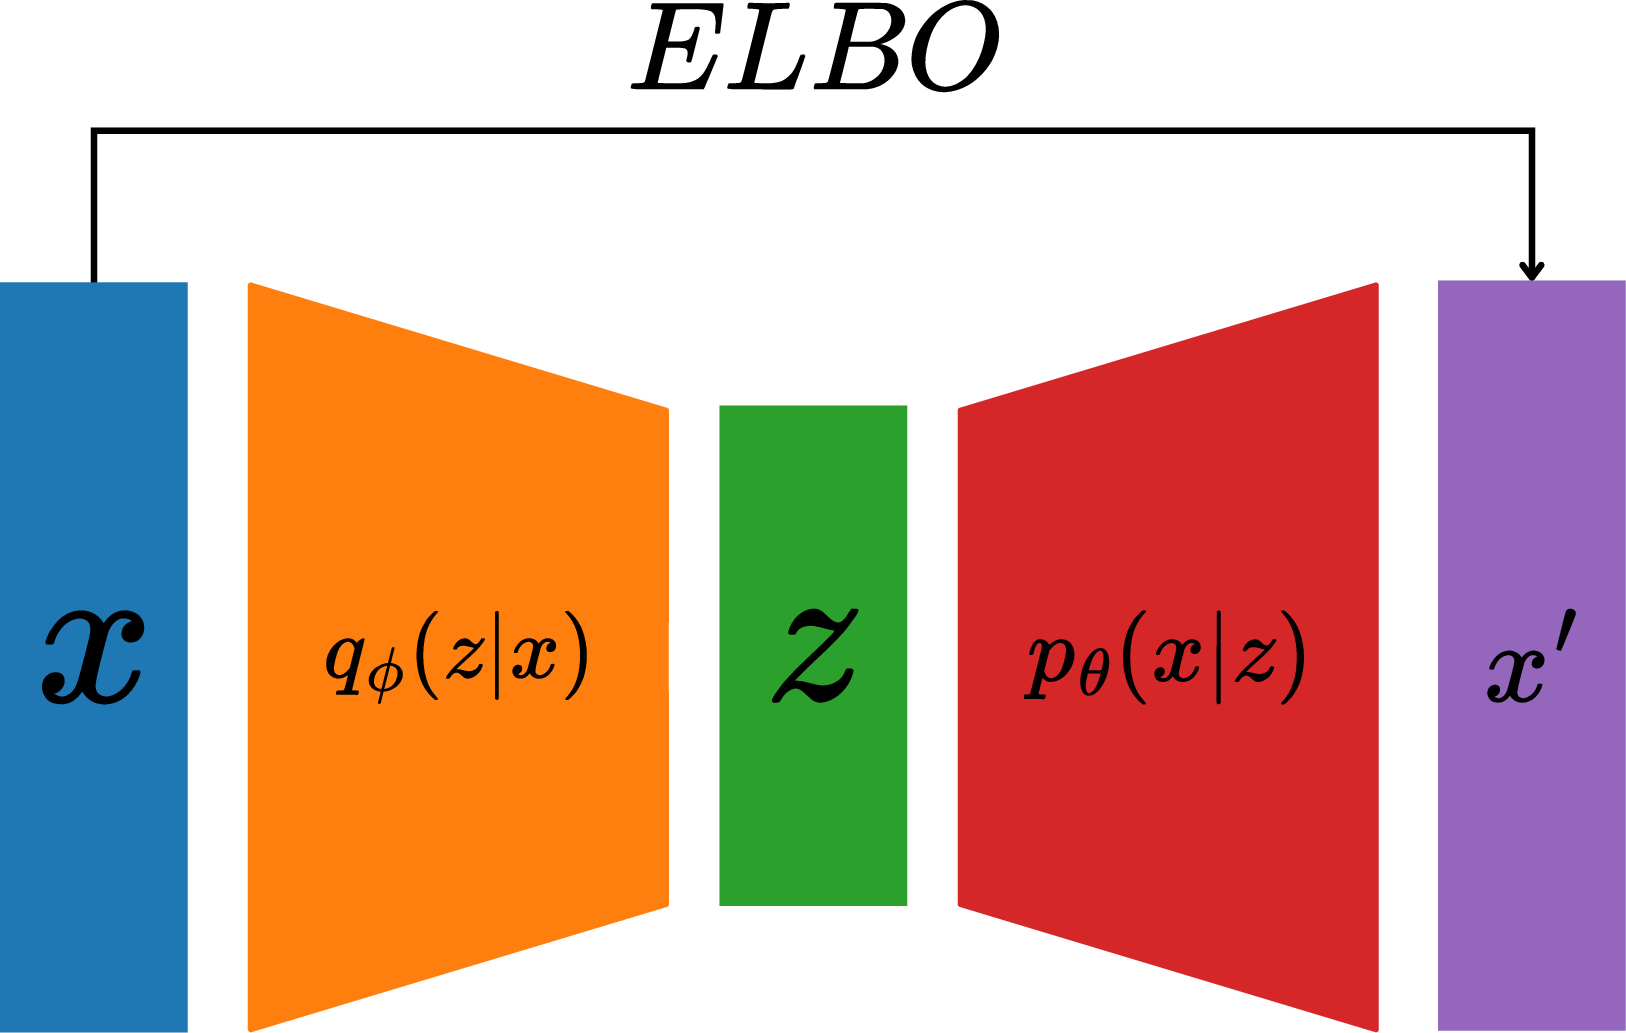
\includegraphics[width=\textwidth]{figures/vae.png}
  \end{minipage}
\end{frame}

\begin{frame}[fragile]
  \frametitle{Our Method}
  We extend the VAE with the following Idea:
  
  Next to $p(z)$ and $p(x | z)$, there is another view of $z$. Namely, the semantic view: $p(y | x, z)$ (Explain why dependent on $x$ and $z$)
  
\end{frame}


\begin{frame}[fragile]
  \frametitle{Experiments}
  
\end{frame}


\begin{frame}
  \frametitle{Slide title}
  \framesubtitle{A frame subtitle}
  Headline of a text slide with enumeration
  \begin{itemize}
    \item Example of an enumeration. This is fake text for illustration. Sitei labores appetere corrumpit, animal urbanitas sit ea.
    \item Example of a second enumeration. This is fake text for illustration. Sitei labores appetere. Qui intellegat mnesarchum.
  \end{itemize}
\end{frame}

\setbeamercolor{structure}{fg=tuescarlet}

\begin{frame}
  \frametitle{Mathematics in your presentation}
  
  Of course you can use mathematical formulas ($a^2+b^2=c^2$) and equations:
  \begin{equation}
    \int_0^\infty \frac{\sin x}{x} \text{d}x=\frac{\pi}{2}.
  \end{equation}
  You can use standard \LaTeX\ beamer commands to change the colours and appearance:
  
  \setbeamercolor{normal text}{fg=black}
  \setbeamercolor{math text}{fg=tuescarlet}
  \setbeamertemplate{itemize items}[default]         % itemize item symbols
  \setbeamercolor{structure}{fg=tuescarlet}          % itemize bullets
  \setbeamercolor{itemize/enumerate body}{fg=black}  % itemize text colour
  
  \begin{itemize}
    \item Black text,
    \item Scarlet formulas: $a^2+b^2=c^2$.
  \end{itemize}
\end{frame}

\setbeamercolor{structure}{fg=tuedarkblue}  % reset the color for itemize bullets

\title{} % to remove the title from the footer
\begin{frame}
  \frametitle{Example of a text slide in two columns}
  
  \begin{multicols}{2}
    \begin{itemize}
      \item Example of an enumeration. This is fake text for illustration. Sitei labores appetere corrumpit, animal urbanitas sit ea.
      \item Example of a second enumeration. This is fake text for illustration. Sitei labores appetere. Qui intellegat mnesarchum.
      \item Example of an enumeration. This is fake text for illustration. Sitei labores appetere corrumpit, animal urbanitas sit ea.
      \item Example of a second enumeration. This is fake text for illustration. Sitei labores appetere. Qui intellegat mnesarchum.
    \end{itemize}
  \end{multicols}
\end{frame}

\begin{imageframe}[bgimage=rightpic.jpg]
  \twocolumn  % this command makes sure that the title is placed inside the first column, which is useful here
  \frametitle{Another example of a text slide in two columns}
  
  \begin{itemize}
    \item Example of an enumeration. This is fake text for illustration. Sitei labores appetere corrumpit, animal urbanitas sit ea.
    \item Example of a second enumeration. This is fake text for illustration. Sitei labores appetere.
          \newpage  % go to the next column (which is empty in this example)
  \end{itemize}
  
\end{imageframe}
\onecolumn % cancel the \twocolumn command and go back to two-column mode

\begin{chapterframe}
  \frametitle{A chapter title}
  
  This is a chapter slide. It can also contain:
  \begin{itemize}
    \item Regular text
    \item enumerations and itemize environments
    \item math
  \end{itemize}
  \[
    \int_0^\infty \frac{\sin x}{x} \text{d}x=\frac{\pi}{2}.
  \]
\end{chapterframe}


% \begin{frame}
%   \frametitle{TU/e and Company logos}

%   The new TU/e logo is available in different three variants (standard, descriptor line, descriptor stack) and different colours (scarlet, black, white). Here are a few examples:

%   \newlength{\lh}
%   \setlength{\lh}{0.85cm}
%   \begin{center}
%     \begin{tabular}{|c|c|c|c|}
%       \hline
%       
\includegraphics[height=\lh]{TUe-logo-descriptor-line-scarlet-rgb}  & 
%       \includegraphics[height=\lh]{TUe-logo-descriptor-stack-scarlet-rgb} & 
%       \includegraphics[height=\lh]{TUe-logo-scarlet-rgb}                  & 
%       \cellcolor{tuedarkblue}\includegraphics[height=\lh]{TUe-logo-white}     \\
%       \hline
%     \end{tabular}
%   \end{center}

%   In \LaTeX\ it is very convenient to create a TU/e beamer theme based on a combination of a company logo with the TU/e logo according to the new TU/e guide lines. Please check the CEC manual for these guide lines. The most important rule is to use the \emph{main colour} of the company. The next six slides depict some examples.
% \end{frame}

% \definecolor{asmlblue}{HTML}{1f3f7d}
% \company{asmllogo}{asmlblue}
% \renewcommand{\companylogosizemultiplicationfactor}{1}

% \title{A presentation of joint work with ASML}
% \subtitle{}
% \author{Name, function}
% \department{Department or Service}

% \begin{titleframe}[variant=2,bgimage=titlebgimg.jpg]
% \end{titleframe}


% \begin{frame}
%   \frametitle{Slide title}
%   \framesubtitle{A frame subtitle}
%   Headline of a text slide with enumeration
%   \begin{itemize}
%     \item Example of an enumeration. This is fake text for illustration. Sitei labores appetere corrumpit, animal urbanitas sit ea.
%     \item Example of a second enumeration. This is fake text for illustration. Sitei labores appetere. Qui intellegat mnesarchum.
%   \end{itemize}
% \end{frame}

% \begin{chapterframe}
%   \frametitle{A chapter title}

%   This is a chapter slide. It can also contain:
%   \begin{itemize}
%     \item Regular text
%     \item enumerations and itemize environments
%     \item math
%   \end{itemize}
%   \[
%     \int_0^\infty \frac{\sin x}{x} \text{d}x=\frac{\pi}{2}.
%   \]
% \end{chapterframe}


% \company{vanderlandelogo}{black}
% \renewcommand{\companylogosizemultiplicationfactor}{1.5} % for company logos that are too wide
% \title{A presentation of joint work with Vanderlande}
% \subtitle{}
% \author{Name, function}
% \department{Department or Service}

% \begin{titleframe}[variant=2,bgimage=titlebgimg.jpg]
% \end{titleframe}

% \begin{frame}
%   \frametitle{Slide title}
%   \framesubtitle{A frame subtitle}
%   Headline of a text slide with enumeration
%   \begin{itemize}
%     \item Example of an enumeration. This is fake text for illustration. Sitei labores appetere corrumpit, animal urbanitas sit ea.
%     \item Example of a second enumeration. This is fake text for illustration. Sitei labores appetere. Qui intellegat mnesarchum.
%   \end{itemize}
% \end{frame}

% \begin{chapterframe}
%   \frametitle{A chapter title}

%   This is a chapter slide. It can also contain:
%   \begin{itemize}
%     \item Regular text
%     \item enumerations and itemize environments
%     \item math
%   \end{itemize}
%   \[
%     \int_0^\infty \frac{\sin x}{x} \text{d}x=\frac{\pi}{2}.
%   \]
% \end{chapterframe}


\end{document}
